\chapter{Le interfacce utente}

Un'interfaccia è qualcosa che sta fra due facce. E' il punto di contatto fra due sistemi che tentano di comunicare. L'interfaccia serve quindi per
comunicare. Un'interfaccia può essere fisica (pulsanti), grafica (immagini a monitor) o di altre forme come per esempio un interprete, un traduttore
simultaneo o un mediatore culturale. 

Le interfacce possono far comunicare due macchine fra loro come nel caso del processore che tramite l'interfaccia USB scambia dati con la stampante.
Oppure possono far comunicare l’uomo con la macchina, come il cruscotto di un’auto, i cursori di un amplificatore, il rubinetto del lavandino, il
manubrio e i pedali della bicicletta.

Un'interfaccia utente è quindi sempre composta da due parti. Una di queste parti appartiene ad una persona l'altra ad uno strumento. Lo strumento è
ciò che compie l'azione, l’interfaccia è ciò che serve per permettere all'utente di guidare lo strumento nell'esecuzione dell'azione. Per esempio,
in un coltello la lama è lo strumento (che compie l'azione del tagliare), il manico è l’interfaccia che consente all'uomo di usare la lama senza
tagliarsi e quindi di guidare lo strumento in maniera soddisfacente. 

\begin{figure}[!h]
	\centering
	\includegraphics[scale=0.8]{immagini/interfaccia.png}
	\caption{Il manico è un esempio di interfaccia.}
\end{figure}


Quando parliamo di \textbf{User Interface o UI}, in italiano Interfaccia Utente, parliamo quindi dello spazio (non necessariamente fisico, il dominio
di una interazione ha una dimensionalità pari a quella dei nostri sensi) di un sistema dove avviene l'interazione fra uomo-macchina. Tipicamente,
si parla di UI in ambito informatico e tecnologico e quindi le interfacce utente sono comunemente identificate come sistemi atti a mettere in
comunicazione l'uomo con computer, sistemi informatici e oggetti intelligenti.

\vspace{\baselineskip}
\textit{User interfaces are a mapping from the sensory, cognitive, and social human world to these collections of functions exposed by a computer
program.}

[Amy J. Ko]
\vspace{\baselineskip}

L'obiettivo primario dell'interazione fra uomo e macchina è quello di consentire all'utente di controllare e far funzionare la macchina in modo efficace.
L'interfaccia deve quindi essere progettata per semplificare l'interazione fra l'uomo e la macchina rendendo così l'esperienza d'uso piacevole e
prolifica. L'interazione fra uomo e macchina deve sempre essere facile, efficiente e divertente così da massimizzare la User Experience del prodotto.

E' importante ricordare che l'uomo si è evoluto grazie alla sua capacità di adattamento che ha la sua massima espressione nel libero arbitrio e nella
capacità di prendere decisioni non necessariamente basate sulla logica ma piuttosto sulle sensazioni e intuizioni. Viceversa le macchine hanno un
comportamento puramente deterministico e pertanto non hanno nessuna capacità di adattamento. L'interfacci uomo macchina va quindi ad avere un ruolo
fondamentale nell'interazione fra le parti dal momento che abilita la comunicazione fra due realtà aventi principi e modalità di "funzionamento"
diametralmente opposte.

Un'interfaccia ben progettata consente all'utente di controllare l'apparato richiedendo uno sforzo fisico e cognitivo minimo. La buona interfaccia
massimizza inoltre la quantità di informazioni utili trasferite all'utente durante l'interazione evitando un sovraccarico informativo che provocherebbe
nell'utente confusione e quindi frustrazione.

\begin{figure}[!h]
	\centering
	\includegraphics[width=0.9\textwidth]{immagini/tesla.jpg}
	\caption{Cruscotto della Tesla model S (\href{https://pinxcars.com/2013-tesla-model-s-cockpit/}{\underline{Fonte}}.)}
\end{figure}

Per questo motivo, la progettazione di un'interfaccia è per definizione un'attività interdisciplinare che va oltre la programmazione grafica e
abbraccia la psicologia, le neuroscienze, il design e la fisica.

Le interfacce sono organizzabili secondo livelli. L' \textbf{HID o Human Interface Device} è la periferica grazie al quale l'utente interagisce con
il sistema; come ad esempio mouse, monitor, gamepad, ecc.. Lo \textbf{HMI o Human Machine Interface} è invece un concetto che astrae dall' HID.
Con HMI, si intende infatti, tutto il sistema di interazione uomo macchina che usa l'HID come elemento di contatto fisico con l'utente. Nel computer
per esempio, la HMI è il sistema mouse+cursore+finestre. Il mouse e il monitor sono HID.

Quando la macchina in questione è un computer, HMI diviene \textbf{HCI o Human Computer Interface}.

\section{Classificazione delle interfacce}
Le interfacce utente sono tipicamente organizzate sulla base dei sensi che utilizzano per stabilire l'interazione fra umano e macchina. Gli umani
possiedono cinque sensi (tatto, vista, udito, olfatto e gusto). Questo porta ad identificare cinque categorie di interfacce possibili, più una sesta
che è legata al cosidetto senso dell'equilibrio (balance in inglese) che però non è considerato un senso vero e proprio nella fisiologia umana.

Possiamo quindi organizzare le interfacce in 6 categorie:
\begin{itemize}
	\itemsep-0.3em
	\item \textbf{Tactile UI} (touch, tatto);
	\item \textbf{Visual UI} (sight, vista);
	\item \textbf{Auditory UI} (sound, udito);
	\item \textbf{Olfactory UI} (smell, olfatto);
	\item \textbf{Gustatory UI} (taste, gusto);
	\item \textbf{equilibrial UI} (balance, equilibrio).
\end{itemize}

La maggior parte delle interfacce utente utilizza però più di un senso umano per stabilire il collegamento. Le interfacce che usano più di un senso
sono dette \textbf{CUI o Composite User Interface}. Le più comuni e note CUI sono chiaramente le famose \textbf{GUI o Graphical User Interface},
le quali sono composte da interfacce grafiche (visual) e tattili (tactile). 

Se ad una GUI andiamo ad aggiungere anche il suono otteniamo una \textbf{MUI o Multimedia User Interface}.

Quindi quando ci si riferisce all'interfaccia di una app con il termine GUI spesso compiamo un errore perchè ormai la maggior parte dei dispositivi
informatici ha anche una sorgente sonora che è utilizzata durante l'interazione (feedback audio del touch sullo schermo, per esempio) e quindi ci
troviamo di fronte ad una MUI e non ad una GUI.


È bene sottolineare che \textbf{estendere le interfacce con più canali (sensi) non è sempre una buona idea}.
\begin{figure}[!h]
	\centering
	\includegraphics[scale=0.85]{immagini/flora_video.png}
	\caption{Esempio: video di Facebook (\href{https://www.facebook.com/Lastknight/posts/10158944882367053}{\underline{Fonte}}).}
\end{figure}

Prendiamo ad esempio i video di
Facebook, i video vengono riprodotti di default con l'audio disattivato per aumentare l'usabilità del sistema.
Gli ingegneri di Facebook si sono accorti infatti che la maggioranza delle persone che visualizzando i video, mutavano immediatamente il suono per
varie ragioni (e.g. privacy o utilizzo di Facebook in momenti non opportuni), quindi hanno reso questa opzione di default. Ovviamente se ragionassimo
in termini di capacità e possibilità dell'interfaccia sembrerebbe assurdo bloccare di default l'utilizzo di un canale.
Questo processo di analisi ha portato poi a far evolvere il mondo dei video online inserendo di default i sottotitoli. Siamo quindi in una situazione in
cui per aumentare l'usabilità del sistema se ne riducono le funzionalità (di default).

%Questo, oltre ad essere un ottimo esempio di MUI riprogettata in GUI, è anche un esempio di tecnica ideata per gli utenti disabili e riusata per
%far fruire il prodotto a quelle personas che lo utilizzano in momenti in cui non possono usufruire dell'audio.


\section{Categorizzare le CUI}
Le CUI possono essere categorizzare in tre diverse macrocategorie:

\begin{itemize}
	\itemsep-0.3em
	\item \textbf{Standard}: usano dispositivi standard come tastiere, mouse e monitor
	\item \textbf{Virtual}: Bloccano all'utente l'interazione con il mondo reale e creano un mondo virtuale che funge da interfaccia fra l'utente e
	la macchina.
	\item \textbf{Augmented}: Non bloccano all'utente la percezione del mondo reale ma la vanno ad arricchire. L'interfaccia è quindi un mix di
	contenuti reali e virtuali che vanno ad arricchire la realtà \textbf{espandendola}.
\end{itemize}

\begin{figure}[!h]
	\centering
	\includegraphics[width=\textwidth]{immagini/standard-virtual-interfaces.png}
	\caption{Tipi di interfaccia.}
\end{figure}

Le CUI possono essere anche \textbf{classificate tramite il numero di sensi che utilizzano}. Ad esempio, lo \textit{Smell-O-Vision} è una CUI
standard 3S, cioè è una normale interfaccia di tipo standard che nell'utilizzo coinvolge 3 sensi dell'utente (Visione, Udito e Olfatto). Se si
aggiungesse un quarto senso (per esempio le poltrone mobili dei cinema 4D) diventerebbe 4S.

Quando un'interfaccia utente interagisce con tutti i sensi umani viene chiamata \textbf{Qualia Interface} (il termine ``qualia" deriva
dalla \href{https://it.wikipedia.org/wiki/Qualia}{\underline{teoria filosofica dei qualia}}).

\begin{figure}[!h]
	\centering
	\includegraphics[scale=0.2]{immagini/react.jpg}
	\caption{Esempio di interfaccia aumentata 3S: Microsoft Reactable.}
\end{figure}

\section{Human Interface Devices}

Un ``human interface device" è un dispositivo informatico usato da umani e, tipicamente, prende input da umani; col termine HID si intendono sia i
\textbf{dispositivi fisici} sia il \textbf{protocollo USB-HID}.

\subsection*{Protocollo HID}

Il termine HID è stato coniato da Microsoft per permettere l'innovazione nell'ambito dei dispositivi di input e per semplificare il processo di
installazione di questi dispositivi; prima dell'introduzione dello standard, questi seguivano protocolli che dipendevano dal loro tipo
(mouse, tastiere, joystick etc.): nel caso di nuovi dispositivi, le opzioni erano adeguarsi a un protocollo già esistente o sviluppare
nuovi driver specifici. Invece, i dispositivi HID spediscono pacchetti che ne descrivono il tipo e che contengono dati di svariati tipi e formati.

Un singolo driver HID procede col parsing del pacchetto di dati e permette l'associazione dinamica di dati I/O con le funzionalità del sistema: è
possibile mandare dati come dispositivo standard e, per esempio, lasciare al sistema operativo il compito di decidere come utilizzarli. Il protocollo
ha dei limiti, ma i sistemi operativi moderni riconoscono dispositivi USB HID standard (mouse, tastiera) senza bisogno di driver specifici.

Nel protocollo HID si distinguono due entità:
\begin{itemize}
	\itemsep-0.3em
	\item \textbf{device}: interagisce direttamente con l'umano.
	\item \textbf{host}: comunica col device e riceve dati sulla base delle azioni eseguite dall'umano; i dati in output vanno dall'host al
	device all'umano.
\end{itemize}

Inoltre, il protocollo ha reso molto semplice la costruzione di nuovi dispositivi introducendo il concetto di \textbf{HID descriptor}:
\textbf{è un pacchetto standard che definisce la categoria di appartenenza e la struttura di dato del device} (NON ha bisogno di essere generato
dal dispositivo, può essere hard coded) e che viene inviato non appena il device viene collegato all'host.
Tipicamente, il device salva sulla ROM l'HID descriptor e non ha bisogno di capirlo; infatti, alcuni mouse e tastiere in commercio sono implementate
usando una CPU a 8-bit.

Il ruolo dell'host è più complesso poich\'e ha bisogno di ricevere l'HID descriptor dal device e farne il parsing prima di poter comunicare con questo:
ha bisogno della potenza computazionale necessaria per l'interpretazione del pacchetto.
Essendo chiaro che non tutti gli host potrebbero essere capaci di interpretare l'HID descriptor, HID descrive anche il ``boot protocol": prevedendo
pacchetti di formato predefinito, sono supportati solo alcuni device specifici (solo tastiera e mouse) con alcune feature specifiche.

HID è stato esteso a una serie di protocolli, si riportano alcuni esempi:
\begin{itemize}
	\itemsep-0.3em 
	\item \textbf{Bluetooth HID}: usato per mouse e tastiere connesse via Bluetooth.
	\item \textbf{Serial HID}: usato per telecomandi su Windows Media Center.
	\item \textbf{ZigBee input device}: ZigBee (RF4CE) supporta dispositivi HID attraverso il profilo ZigBee input device.
	\item \textbf{HID over I²C}: usato per dispositivi embedded su Microsoft Windows 8.
	\item \textbf{HOGP} (HID over GATT): usato per dispositivi HID connessi attraverso BLE.
\end{itemize}

\pagebreak
\subsection*{Periferiche HID}

Le periferiche HID sono organizzate in due categorie:
\begin{itemize}
	\itemsep-0.3em
	\item \textbf{di input}: basati su sensori, converte la realtà fisica in segnale elettrici. Un esempio di sensore è un microfono.
	\item \textbf{di output}: basati su attuatori, converte segnali elettrici in perturbazioni nel mondo. Un esempio di attuatore è un altoparlante.
\end{itemize}

Dispositivi di input e di output venivano tradizionalmente divisi in classi sulla base del tipo di input/output usato dall'HID, al giorno d'oggi questa
classificazione tende a decadere poich\'e la maggior parte dei dispositivi moderni usano più tecnologie; di seguito, le classi:
\begin{itemize}
	\itemsep-0.3em
	\item \textbf{testi e caratteri};
	\item \textbf{posizioni};
	\item \textbf{suoni};
	\item \textbf{immagini};
	\item \textbf{parametri ambientali};
	\item \textbf{posizione};
	\item \textbf{parametri fisiologici e biologici}.
\end{itemize}

\subsubsection*{HID testi e caratteri}
L'HID della classe testi e caratteri più comune è la \textbf{tastiera}.
Tre layout sono da prendere in considerazione per le tastiere:
\begin{itemize}
	\itemsep-0.3em 
	\item \textbf{layout fisico}: corrisponde al posizionamento dei tasti sulla tastiera. \`E normato.
	\item \textbf{layout visuale}: corrisponde all'arrangiamento dei simboli che appaiono sui tasti. Ad esempio, qwerty, azerty etc.
	\item \textbf{layout funzionale}: corrisponde all'associazione tasto-significato all'interno di un software. Ad esempio, quando si apre YouTube
	viene messo a disposizione un layout funzionale in cui alla barra spaziatrice si fa corrispondere riproduzione e pausa.
\end{itemize}

\begin{figure}[!h]
	\centering
	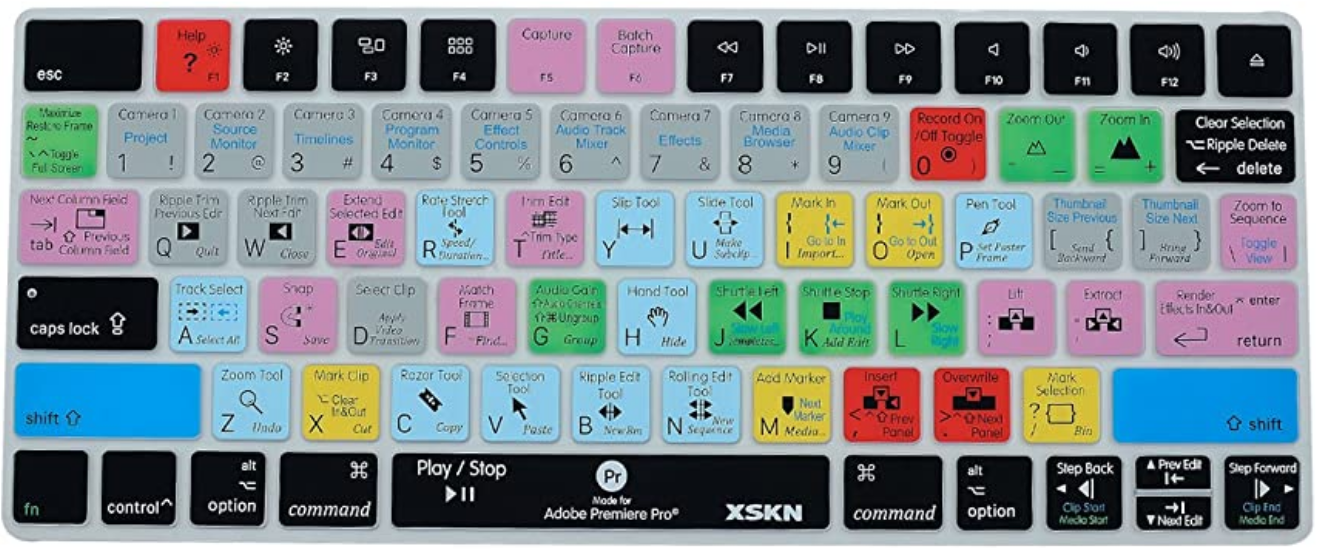
\includegraphics[scale=0.25]{immagini/adobe-layout-funzionale.png}
	\caption{Esempio di layout funzionale di una tastiera su Adobe Premiere Pro.}
\end{figure}

Esistono inoltre \textbf{tastiere multifunzione}, che estendono tastiere standard con altri tasti e mappature; necessitano di driver aggiuntivi a meno
che il produttore non le faccia apparire come una tastiera standard estesa e poi deleghi a un applicativo il compito di associare un layout funzionale
appropriato.

Un altro dispositivo HID testi e caratteri è il \textbf{lettore di codice a barre}: concretamente, è un serializzatore di caratteri. Un codice QR è un
\textbf{barcode} bidimensionale che usa quattro modalità di encoding per salvare i dati in modo efficiente.

I \textbf{tag RFID} sono formati da un transponditore radio (cioè un trasmettitore e un ricevitore radio); ne esistono di \textbf{passivi} (fanno
energy harvesting, prendono la potenza dall'onda elettromagnetica che impatta con l'antenna dell'host; l'antitaccheggio dei negozi usano un RFID passivo)
e di \textbf{attivi} (usano una batteria e si usano tipicamente per la geolocalizzazione).

\textbf{NOTA BENE}. RFID e NFC non sono la stessa cosa: NFC permette comunicazioni bidirezionali, non è per solo input.

\subsubsection*{Sistemi di puntamento}
Sono dispositivi di input che trasferiscono input di tipo spaziale verso un computer: i movimenti fisici dell'utente vengono replicati su uno schermo
attraverso movimenti di un puntatori e/o altri cambiamenti visivi.

Si definisce in merito la \textbf{legge di Fitt} per il calcolo del tempo di movimento MT: \( MT = a + b * ID = a + b * \log_2 \frac{2D}{W} \)

con \textbf{a} definito come il tempo (in secondi) necessario per iniziare o smettere di muoversi (si misura empiricamente per ciascun dispositivo),
\textbf{b} la velocit\`a del dispositivo (si misura empiricamente per ciascun dispositivo),
\textbf{D} la distanza dal punto iniziale al centro dell'obiettivo,
\textbf{W} la larghezza dell'obiettivo misurata lungo l'asse su cui ci si sta muovendo.

Si danno i seguenti criteri per la classificazione di dispositivi di puntamento:
\begin{itemize}
	\itemsep-0.3em
	\item sulla base del \textbf{tipo di input}:
	\vspace{-3mm}
	\begin{itemize}
		\itemsep-0.3em
		\item \textbf{diretto} se il puntatore si trova nella stessa posizione fisica che il device (ad esempio, il dito su un touch screen);
		\item \textbf{indiretto} quando traduce il movimento sullo schermo (ad esempio, il mouse o lo stilo di una tavoletta grafica).
	\end{itemize}
	\item sulla base del \textbf{modo in cui il movimento viene mappato} sull'interfaccia:
	\vspace{-3mm}
	\begin{itemize}
		\itemsep-0.3em
		\item \textbf{assoluto} quando il mapping tra lo spostamento nel mondo fisico viene replicato così com'è sul dispositivo;
		\item \textbf{relativo} altrimenti.
	\end{itemize}
	\item sulla base di \textbf{come} i dispositivi producano il segnale sulla base dello spostamento:
	\vspace{-3mm}
	\begin{itemize}
		\itemsep-0.3em
		\item \textbf{isotonico} (stesso tono), si può muovere nello spazio e misura lo spostamento;
		\item \textbf{isometrico} (stesso metro), è fisso e misura la forza che viene applicata;
		\item \textbf{elastico}, la forza applicata è proporzionale allo spostamento (ad esempio, il joystick a molla).
	\end{itemize}
	\item sulla base della \textbf{velocità con cui si fa avanzare il puntatore}:
	\vspace{-3mm}
	\begin{itemize}
		\itemsep-0.3em
		\item \textbf{position control}, si controlla la posizione (relativa o assoluta) del puntatore;
		\item \textbf{rate control}, si controlla la velocità e la direzione del puntatore (ad esempio, i joystick degli arcade games).
	\end{itemize}
\end{itemize}

Di seguito verranno elencati dispositivi di puntamento innovativi.

I dispositivi \textbf{eye tracker} misurano la posizione della pupilla e i movimenti degli occhi, sono usati tipicamente nella ricerca. Ci sono vari
modi per estrarre l'informazione sulla posizione della pupilla:

\begin{figure}[!h]
	\centering
	\begin{subfigure}[!h]{0.3 \textwidth}
		\centering
		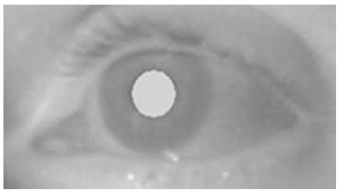
\includegraphics[scale=0.15]{immagini/bright-pupil.png}
		\caption{Metodo bright pupil.}
	\end{subfigure}
	\begin{subfigure}[!h]{0.3 \textwidth}
		\centering
		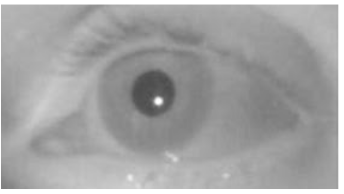
\includegraphics[scale=0.15]{immagini/dark-pupil.png}
		\caption{Metodo dark pupil.}
	\end{subfigure}
	\begin{subfigure}[!h]{0.3 \textwidth}
		\centering
		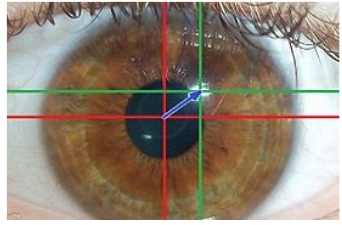
\includegraphics[scale=0.15]{immagini/passive-light.png}
		\caption{Metodo passive light.}
	\end{subfigure}
\end{figure}

\begin{itemize}
	\itemsep-0.3em
	\item \textbf{bright-pupil}: la sorgente illumina con luce infrarossa la pupilla, è coassiale col punto di vista.
	\item \textbf{dark-pupil}: la sorgente illumina con luce infrarossa la pupilla, non è coassiale col punto di vista.
	\item \textbf{passive light}: usa la luce ambientale, il consumo energetico è minimo.
\end{itemize}

Si ricorda inoltre la differenza tra eye tracking e \textbf{gaze tracking}: il secondo si occupa di capire dove il soggetto stia guardando
riportando l'angolo della pupilla nello spazio tridimensionale in cui è inserito il soggetto (sono dunque necessarie anche angolo e posizione
di testa e soggetto). Per rendere l'eye tracking un sistema di puntamento, questo va abbinato al gaze tracking; in merito, ci sono due
possibilità: o si monitora la posizione della testa o si vincola la testa a un supporto.

I dispositivi \textbf{dataglove} sono dei guanti che consentono di estrarre informazioni sulla posizione delle dita e l'orientamento triassiale
della mano.

I \textbf{dispositivi aptici} sono dispositivi input/output che permettono agli utenti di toccare, percepire e manipolare oggetti tridimensionali
in ambienti virtuali (restituendo sensazioni tattili); sono usati nelle simulazioni, nel CAD 3D e in ambito medico.

Altri esempi sono \textbf{smart papers} e \textbf{lavagne digitali}.

\subsubsection*{Dispositivi per il suono}
Un \textbf{microfono} è un dispositivo che converte un suono in un segnale elettrico.

Un \textbf{array di microfoni} è un insieme di microfoni (tipicamente omnidirezionali) che opera in tandem, permette di riconoscere la direzione
di provenienza dei suoni, cancellare eco e/o background noise. Dopo una trasformazione dei dati (attraverso dei microcontrollori detti DSP), l'obiettivo
è creare uno o più microfoni virtuali.

Si parla molto di \textbf{interfacce vocali}, inadatte però alla maggior parte delle applicazioni: l'obiettivo in termini di design è quello di abbassare
il carico cognitivo necessario all'utente per interagire con la piattaforma, ma la larghezza di banda (intesa come la quantità di dati trasferibile) con
un'interfaccia vocale è di molto inferiore a quella di una GUI.

\subsubsection*{Sensori di immagini}
Un \textbf{sensore di immagini} è un digitalizzatore di radiazioni luminose, converte radiazioni luminose in una rappresentazione cromatica (tipicamente
RGB). I sensori più comuni sono i CMOS: array di capacitori che vengono caricati o scaricati a seconda dell'attivazione del fotodiodo che viene
impattato dalla radiazione luminosa, per ogni pixel si hanno 3 elementi sensibili, uno per il rosso, uno per il giallo e uno per il blu.

Il \textbf{3D scanning} consiste nel rappresentare dimensione e posizione nello spazio tridimensionale di oggetti e ambienti, l'obiettivo principale
è ricostruire la forma degli oggetti (il colore è secondario). Si distinguono due categorie di scanner 3D:
\begin{itemize}
	\itemsep-0.3em 
	\item \textbf{passivi}: non emettono radiazioni elettromagnetiche, si affidano all'illuminazione ambientale. Di seguito, alcuni esempi:
	\vspace{-3.mm}
	\begin{itemize}
		\itemsep-0.3em
		\item \textbf{camere stereoscopiche}: usano due camere poste a una distanza focale simile a quella dell'occhio umano e, calcolando la differenza
		nelle immagini pixel per pixel, creano una terza immagine detta ``depthmap" per creare l'illusione della profondità.
		\item \textbf{sistemi fotometrici}: assumono l'esistenza di una sorgente luminosa controllabile e analizzando gli spostamenti delle ombre al variare
		dell'incidenza (della sorgente luminosa) vengono calcolati sia la profondità sia il colore.
		\item \textbf{tecniche silhouette}: tipicamente messe a disposizione anche da applicazioni per dispositivi mobili, scattando più foto dello stesso oggetto
		da diversi angoli e usando l'accelerometro e la piattaforma iniziale posizionano i piani immagini nello spazio tridimensionale e
		``ricostruiscono'' l'oggetto.
	\end{itemize}
	\item \textbf{attivi}: emettono radiazioni elettromagnetiche, tipicamente vengono usate luci, ultrasuoni o raggi x. Di seguito, alcuni esempi:
	\vspace{-3.mm}
	\begin{itemize}
		\itemsep-0.3em
		\item \textbf{time-of-flight}: inviano un impulso laser (tipicamente nell'infrarosso) e misurano il tempo di ritorno, sono estremamente precisi
		e misurano una distanza punto-punto. La tecnologia per il calcolo del tempo di ritorno è spesso interferometrica.
		\item \textbf{triangolazione}: inviano un impulso laser, usando l'angolo di riflessione e il disallineamento ottico tra emettitore e ricevitore,
		permettono di ricostruire la distanza punto-punto. La tecnologia è più semplice che per time-of-flight.
		\item \textbf{scanner 3D a luce strutturata}: proiettano una immagine geometricamente nota su un oggetto tridimensionale e analizzano la
		deformazione indotta dall'oggetto sull'immagine per ricostruire la forma dell'oggetto (non è punto-punto, restituisce una depthmap). Viene usato
		dal Kinect di Microsoft.
		\item \textbf{scanner 3D a luce modulata}: proiettano una immagine che ha punto-punto una proprietà di frequenza diverse (concretamente, è come
		fare time-of-flight in parallelo su più punti). \`E una tecnica molto poco usata.
	\end{itemize}
\end{itemize}

\subsubsection*{Dispositivi wearable}
Si definisce \textbf{wearable device} un sistema in cui la parte sensoriale, di interfaccia e di computing sono tutte riunite e vengono indossate
dall'utente (ad esempio, uno smartwatch è un dispositivo wearable, un paio di cuffie bluetooth invece no) e sono tipicamente molto specializzati
(per esempio, è il caso dei fitness trackers). I problemi tecnici principali sono il consumo di batteria e la dissipazione del calore, entrambi accentuati
dal fatto che questi dispositivi dovrebbero restare costantemente attivi.

Un dispositivo \textbf{heart rate monitor} permette di misurare il battito cardiaco dell'utente utilizzando dei \textbf{sensori PPG}: illuminando
tipicamente un polpastrello o il polso e analizzando l'immagine riflessa, vengono estratte informazioni sulla quantità di sangue
(NOTA: invece, i sensori ECG usano dei segnali elettrici per misurare l'espansione e la contrazione del muscolo cardiaco).

Un dispositivo \textbf{EEG headset} permette di monitorare gli impulsi elettrici del cervello posizionando elettrodi non-invasivi sullo scalpo, questi
vengono poi amplificati e digitalizzati per essere processati da un calcolatore; sono tipicamente usati come sistemi di puntamento da utenti disabili.